\chapter{Steering}
The control of steering wheel take advantage of motor for steering assist originally present in the car. The motor is controlled by a positioning controllers designed for brushed DC and brushless DC motors with encoders. denominated \gls{EPOS} by many manufactures

\section{Maxon EPOS 70/10 controller}
\begin{figure}[h]
	\centering
	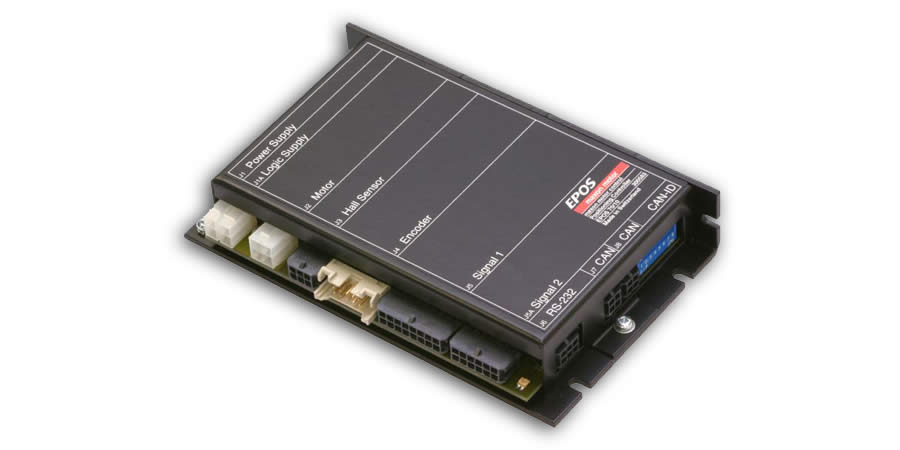
\includegraphics[width=0.5\linewidth]{figures/EPOS-70-10-10-A-11-70VDC-Detail.jpg}
	\caption{Maxon EPOS 70/10 controller}
	\label{fig:maxon_epos}
\end{figure}
The controller available to use is the \href{https://www.maxonmotor.com/maxon/view/product/control/Positionierung/300583}{Maxon EPOS 70/10}. It includes CAN network interface and a RS-232. The relevant electrical specs can be seen in table \ref{tab:epos_specs}. The full specifications as well as connections layout must be seen in \cite{epos_hardware}. The controller contains two led in a single package that is used as status reference. Table \ref{tab:maxon_led_status} present the status of device based on pattern of leds shown by it.

\begin{table}[hb]
	\centering
	\begin{tabular}{lccc}
		\toprule
		\textbf{Description} & \textbf{Min.} & \textbf{Max.} & \textbf{Unity}\\
		\midrule
		Power supply voltage $\text{V}_\text{CC}$ (Ripple \textless 10\%) & 11 & 70 & $\text{V}_\text{DC}$\\
		Max. output voltage & & $0.9\cdot\text{V}_\text{CC}$ & $\text{V}_\text{DC}$\\
		Max. output current $\text{I}_\text{max}$ (\textless 1sec) &  & 25 & A\\
		Continuous output current $\text{I}_\text{cont}$ & & 10 & A\\
		Sample rate PI - current controller &10K & 10K & Hz\\ 
		Sample rate PI - speed controller  &1K & 1K & Hz\\ 
		Sample rate PI - positioning controller &1K & 1K & Hz\\
		Max. speed (motors with 2 poles) & & 25K & rpm\\
		\bottomrule
	\end{tabular}
    \caption{EPOS electric specifications}
    \label{tab:epos_specs}
\end{table}

\begin{table}
	\centering
	\begin{tabular}{p{0.7\textwidth}cc}
		\toprule
		\textbf{Description} & \textbf{Red} & \textbf{Green}\\
		\midrule
		\begin{minipage}{0.4\linewidth}
			The EPOS is in state:
			\begin{itemize}
				\item Switch ON Disabled
				\item Ready to Switch ON
				\item Switched ON
				\item The power stage is disabled
			\end{itemize} 
		\end{minipage} & OFF & Blinking ($\approx$ 1Hz)\\
	    \midrule
	    \begin{minipage}{0.5\linewidth}
	    	The EPOS is in state:
	    	\begin{itemize}
	    		\item Operation Enable
	    		\item Quick Stop Active
	    		\item The power stage is enabled
	    	\end{itemize} 
	    \end{minipage} & OFF & ON\\
        \midrule
        EPOS is in Fault State & ON & OFF\\
        \midrule
        EPOS is in temporary state Fault Reaction Active & ON & ON\\
        \midrule
        There is no valid firmware on the EPOS (due to a failed firmware download) & ON & Flashing \\ 
		\bottomrule
	\end{tabular}
	\caption{Maxon EPOS 70/10 Led status}
	\label{tab:maxon_led_status}
\end{table}
\section{Steering sensor support}
Maxon EPOS 70/10 accepts quadrature sensors to give feedback of position. The used sensor is a quadrature line driver with index (although index is disabled because its track is damaged). The sensor model is HEDR-55L2-BY09 with main characteristics shown in table \ref{tab:quad_sensor} \cite{hedr_sensor}. Table \ref{tab:quad_sensor_settings} show the required configuration to be passed to EPOS device to correctly use the steering controller. See appendix \ref{appendix:maxon} for further description.
\begin{table}[!hb]
	\centering
	\begin{tabular}{lc}
		\toprule
		\textbf{Description} & \textbf{Value}\\
		\midrule
		Line Driver & Yes\\
		Counts per revolution & 3600\\
		Total number of positions & 14400\\
		Shaft diameter & 8mm\\
		\bottomrule
	\end{tabular}
	\caption{Main HEDR-55L2\_BY09 sensor characteristics}
	\label{tab:quad_sensor}
\end{table}

\begin{table}[!hb]
	\centering
	\begin{tabular}{lc}
		\toprule
		\textbf{Description} & \textbf{Value}\\
		\midrule
		Sensor Type & 2\\
		Pulse Number & 3600\\
		Sensor Polarity & 0\\
		\bottomrule
	\end{tabular}
	\caption{Quadrature sensor settings configured in EPOS}
	\label{tab:quad_sensor_settings}
\end{table}

\section{Calibration process}
Here is assumed the vehicle follows a model of Ackermann steering model typical valid for low speed which result in the simplified approximation of the single line model or as in general described in literature as bicycle model.\cite{Snider2009} \cite{Navigation_System_Design} An simplified representation of model is present in figure \ref{fig:ackermann_steering}
\begin{figure}[!hb]
	\centering
	\subcaptionbox{Four wheel representation}{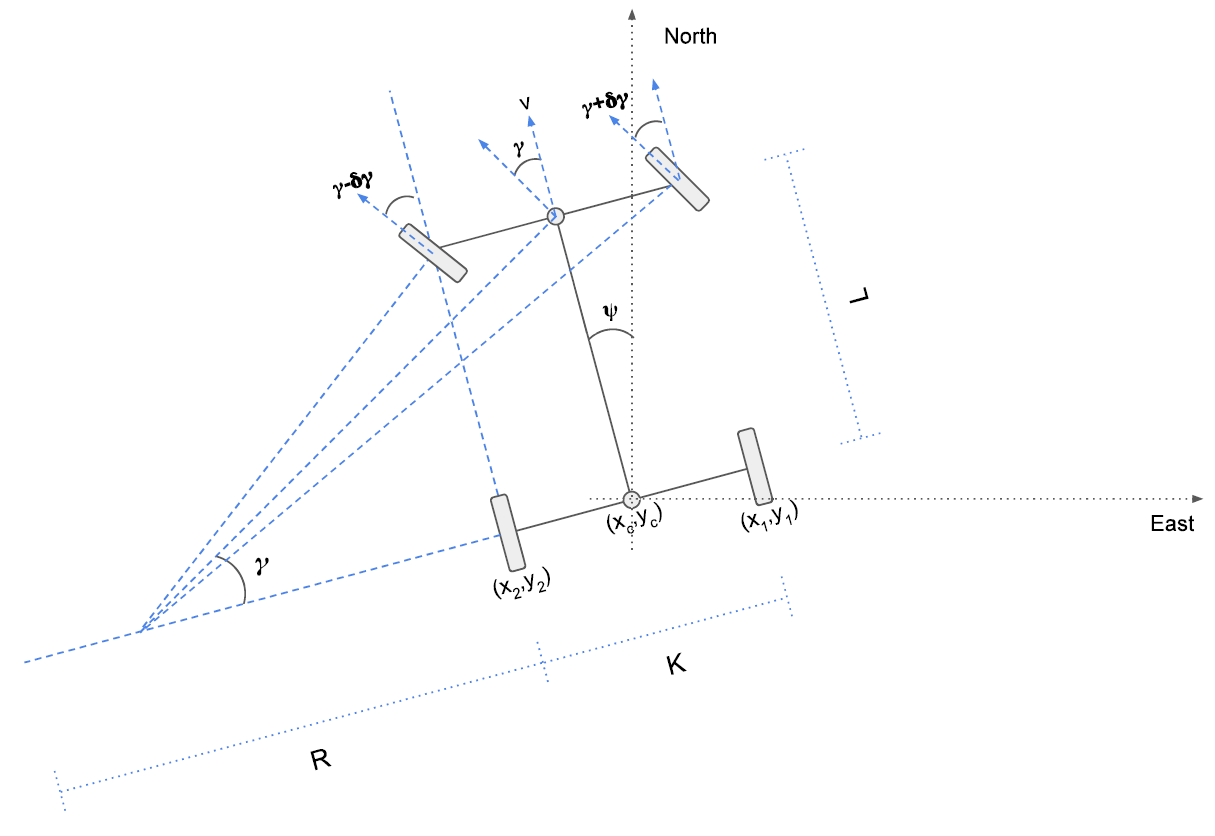
\includegraphics[width=0.7\linewidth]{figures/Ackermann_steering.png}}
	\hfill
	\subcaptionbox{Bicycle Representation (source \cite{Snider2009})}{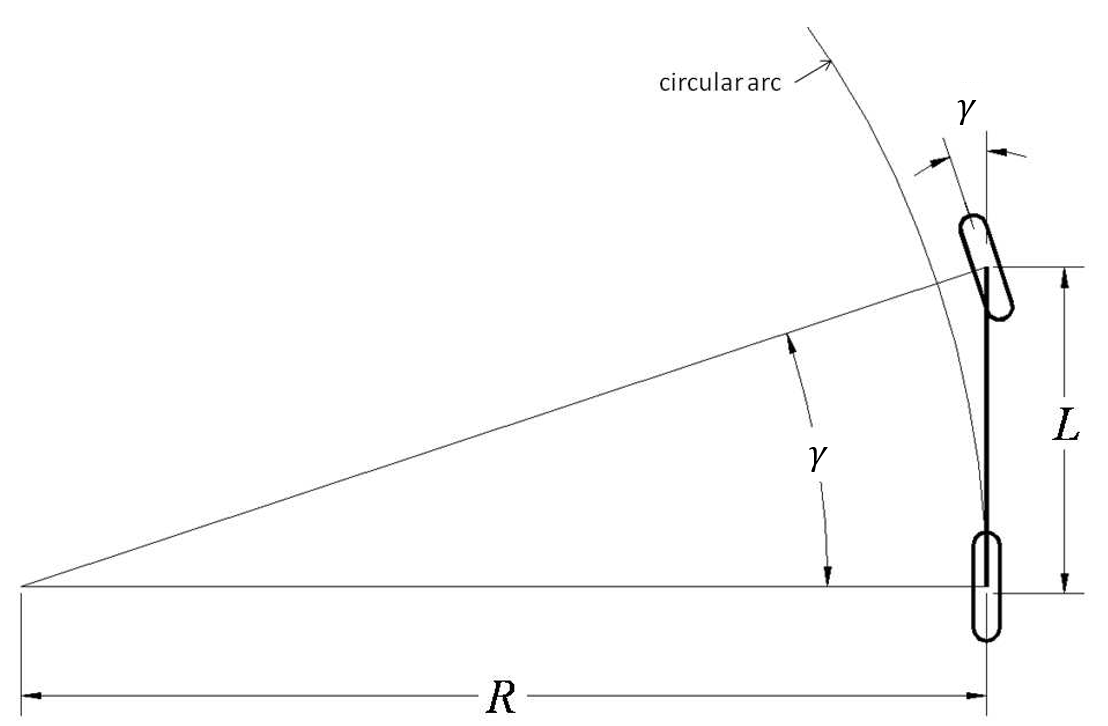
\includegraphics[width=0.5\linewidth]{figures/bicicle_model}}
	\caption{Ackermann steering model simplification}
	\label{fig:ackermann_steering}
\end{figure}
\section{interface library}
\blindtext